%  Template for ICASSP-2021 paper; to be used with:
%          spconf.sty  - ICASSP/ICIP LaTeX style file, and
%          IEEEbib.bst - IEEE bibliography style file.
% --------------------------------------------------------------------------
\documentclass{article}
\usepackage{spconf,amsmath,graphicx,hyperref}

% Example definitions.
% --------------------
\def\x{{\mathbf x}}
\def\L{{\cal L}}

% Title.
% ------
\title{AIML 425 Assignemnt 3}
%
% Single address.
% ---------------
\name{Quan Zhao (Student ID: 300471028)}
%\name{Author(s) Name(s)\thanks{Thanks to XYZ agency for funding.}}
\address{Victoria University of Wellington}


\begin{document}
%\ninept
%
\maketitle
%
\section{Introduction}
\label{sec:intro}

Graph Neural Networks (GNNs) are specialized machine learning models designed to handle graph-structured data. Unlike traditional neural networks, GNNs operate on nodes and edges to capture complex relationships. They work through a process of message passing, aggregation, and feature updating to make predictions or decisions. GNNs are widely used in applications like social network analysis, molecular chemistry, and recommendation systems.

In this work, I will present my understanding of GNN by resolve the "Tiger random walk" problem:

There are 1024 tiger sensors in a square grid in a 3.2 km
by 3.2 km observation area. A tiger enters the area, and then
walks randomly from a sensor to one of eight neighboring
sensors, until it walks out of the area. A fraction $F \in [0, 1]$ of
the sensors does not work. The density of the sensor score s is

\begin{itemize}
  \item $p(s | \text{tiger passed by}) = 1, \quad s \in [0, 1]$
  \item $p(s | \text{no tiger passed by}) = \begin{cases} \frac{2s}{c}, & 0 \leq s < c \\\frac{2(1 - s)}{1 - c}, & c \leq s \leq 1 \end{cases}$
  $\\,\text{(Start with  c = 0 ).}$
\end{itemize}



\section{THEORY}
\label{sec:theory}

\subsection{Graph Convolutional Network (GCN)}
\label{ssec:gcn}
Graph Convolutional Network (GCN) \cite{kipf2016semi} originates from simplifying “proper” graph convolution based on graph Fourier transform
 
\begin{align}
  h_{v}^{t}=\sigma \left ( 
    W^t
    \sum_{u\epsilon N_v\bigcup v}
    \frac{1}{\left | N_v \right |} 
    h_{v}^{t-1}
    \right )
\end{align}

A GCN is well-suited for this problem due to its ability to aggregate local neighborhood information, its simplicity and computational efficiency, its capability to incorporate node features, and its scalability to large graphs.

\subsection{Binary Cross-Entropy (BCE) Loss}
\label{ssec:bce}

Binary Cross-Entropy (BCE)\cite{domingos2012few}  Loss, also known as log loss, is a commonly used loss function for binary classification problems. It quantifies how well the predicted probabilities align with the actual labels.

\begin{align}
  \text{BCE} = -\frac{1}{N} \sum_{i=1}^{N} [y_i \log(\hat{y}_i) + (1 - y_i) \log(1 - \hat{y}_i)]
\end{align}

BCE loss is ideal for this work because it's tailored for binary classification and outputs probabilities, making it compatible with the GNN model. It performs well with imbalanced classes, is differentiable for gradient-based optimization, and is both simple and effective.

\subsection{F1-Score}
\label{ssec:f1}

The F1-score is a metric that combines both precision and recall into a single value, providing a balanced measure of a model's performance on a binary classification task.

\begin{align}
  \text{F1-Score} = 2 \times \frac{\text{Precision} \times \text{Recall}}{\text{Precision} + \text{Recall}}
\end{align}

\begin{align}
  \text{Precision} = \frac{\text{True Positives}}{\text{True Positives} + \text{False Positives}}
\end{align}

\begin{align}
  \text{Recall} = \frac{\text{True Positives}}{\text{True Positives} + \text{False Negatives}}
\end{align}

If the tiger's track covers only a small portion of the grid, most of the sensors will have a label of 0 (tiger didn't pass by). In such cases, the class distribution is imbalanced, and metrics like accuracy can be misleading. F1-score is a better metric for imbalanced datasets.

\section{RESULTS}
\label{sec:results}

\subsection{Data Preparation}
\label{ssec:data}
To resolve "Tiger random walk" problem. 
The first step is to generate data following the requirements.

In practice, we generate data set by

\begin{enumerate}
  \item A 32 * 32 matrix grid, with $F$ percentage node set as sensor failed.
  \item Tiger's track, by random walk in grid, from edge until reach any other edge.
        \\ Set y label for each node based on the track, if on the track set 1, otherwise set 0.
  \item Update the sensor score $x$ using a probability function of $s$, based on whether the node is on track or not.
\end{enumerate}

The Figure $\ref{fig:data}$ (a) shows a random path the node on track shows red color.
Figure $\ref{fig:data}$ (b) shows scores of nodes, , where larger values correspond to darker colors.

\begin{figure}[htb]
  \begin{minipage}[b]{1.0\linewidth}
    \centering
    \centerline{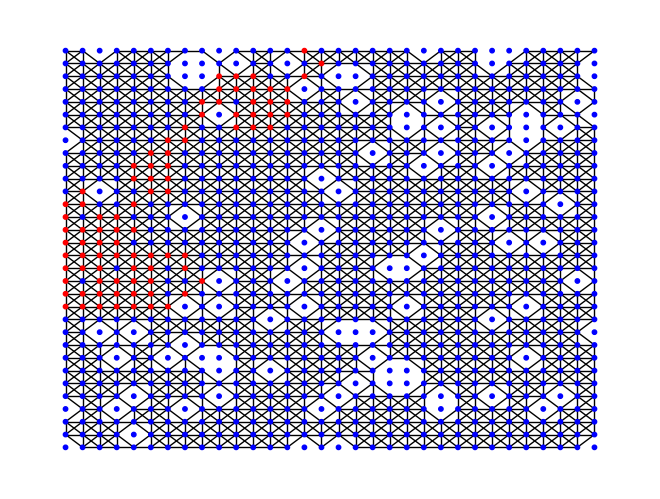
\includegraphics[width=4.0cm]{images/path}}
  %  \vspace{1.5cm}
    \centerline{(a) path of in grid}\medskip
  \end{minipage}
  \hfill
  \begin{minipage}[b]{1.0\linewidth}
    \centering
    \centerline{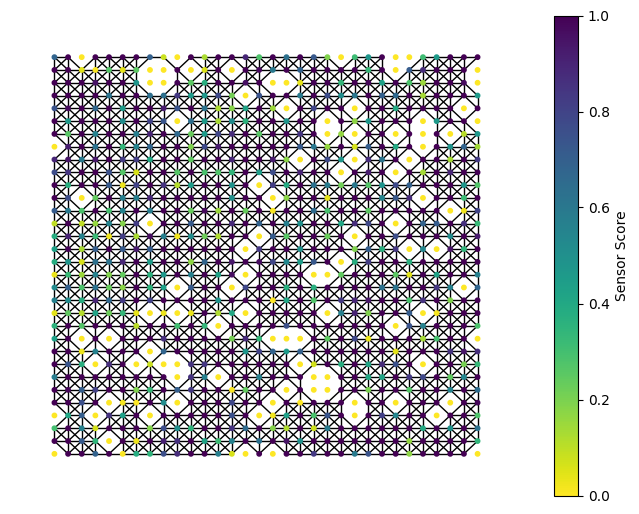
\includegraphics[width=4.0cm]{images/scores}}
  %  \vspace{1.5cm}
    \centerline{(b) node scores in grid }\medskip
  \end{minipage}
  %
  \caption{visulization of dataset}
  \label{fig:data}
  %
  \end{figure}

  \subsection{Model Training and evaluation}
  \label{ssec:model}

  In the model training stage, we generate the dataset by following the approach described above. We then split this dataset into training and testing sets.

  We train the model using a 2-layer GCN (Graph Convolutional Network) on the training dataset. The objective function used is Binary Cross-Entropy (BCE) Loss.
  For evaluation, we compute the F1-scores on the test dataset.

  Finally, we measure track accuracy on the test data for various known values of $F$ and $c$.

  The selected values for $F$ are $0, 0.25, 0.75, 1$, and for $c$, the selected values are $1e-09, 0.0017, 0.0032, 0.0056, 1$.
  
  \begin{figure}[htb]

    \begin{minipage}[b]{1.0\linewidth}
      \centering
      \centerline{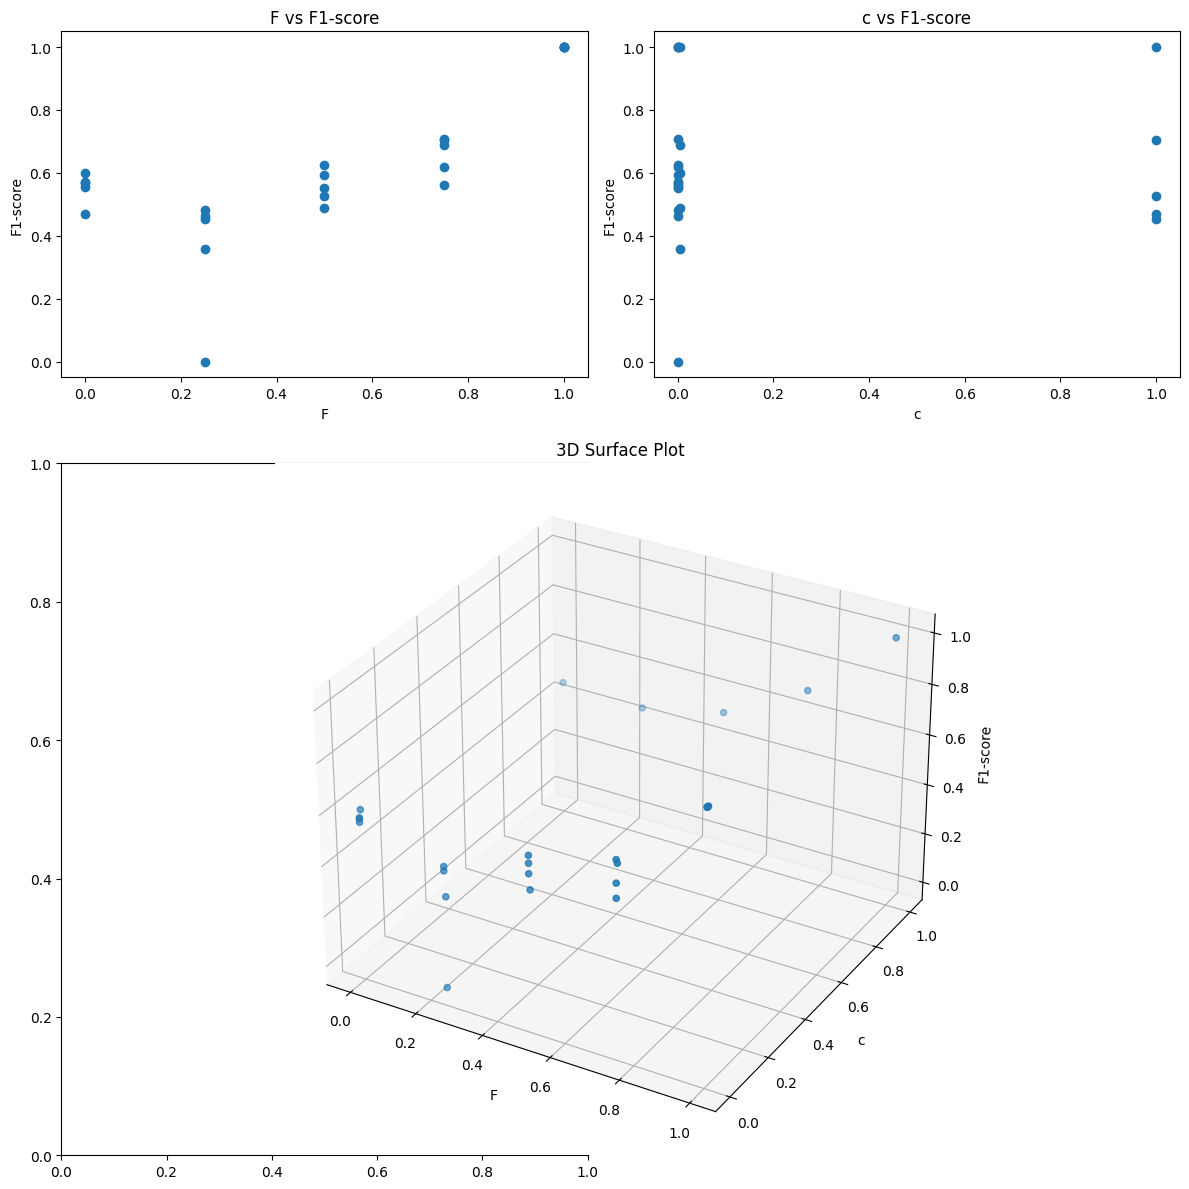
\includegraphics[width=4.0cm]{images/F_c_f1}}
    %  \vspace{2.0cm}
      %\centerline{(a) Result 1}\medskip
    \end{minipage}
    %
    \caption{F1-score distribution with F and c}
    \label{fig:f1}
    %
    \end{figure}


Figure $\ref{fig:f1}$ shows the F1-score value's relationship with F and c score.
Based on the plot results, it appears that the F1-score is affected only when the value of $c$ is close to 0 or 1. For other values of $c$, there seems to be no significant impact on the F1-score.

When $c$ is zero, there is a positive correlation between the F1-score and the value of $F$.
when $c$ is one, the F1-score reaches its lowest point at 
$F$=0.025; beyond that point, both $F$ and the F1-score grow together.

\section{CONCLUSION}
\label{sec:conclusion}

Graph Neural Networks (GNNs) have a wide range of popular applications. Their ability to efficiently resolve the 'Tiger random walk' problem demonstrates that GNNs can effectively handle node classification tasks.

Experimental results indicate that the model's performance is correlated with the node failure rate. However, it is not highly sensitive to variations in the sensor score.

\section{STATEMENT OF ALL TOOLS USED}
\label{sec:statementofalltoolsused}

In this work, we used Pytorch geometric package to generate data, create, train models. 
The Plotly package helped us visualize in 3D. 

Source codes are published in github: 
$\href{https://github.com/felixzhao/AIML425-ASSN-3/blob/main/AIML425_Assignment_3.ipynb}{URL}$
 (runable in google colab)





% To start a new column (but not a new page) and help balance the last-page
% column length use \vfill\pagebreak.
% -------------------------------------------------------------------------
%\vfill
%\pagebreak

\vfill\pagebreak

% References should be produced using the bibtex program from suitable
% BiBTeX files (here: strings, refs, manuals). The IEEEbib.bst bibliography
% style file from IEEE produces unsorted bibliography list.
% -------------------------------------------------------------------------
\bibliographystyle{IEEEbib}
\bibliography{strings,refs}

\end{document}
